\singlespacing
\chapter{Le Grand Collisionneur de Hadrons (LHC) et le détecteur
  ATLAS}
\label{sec:lhc_atlas}
\doublespacing{}

\section{Le LHC}
\label{sec:lhc_atlas:lhc}

% intro
Le Grand Collisionneur de Hadron~\cite{evans_lhc_2008}, noté
LHC~\footnote{De l'anglais, \emph{Large Hadron Collider}}, est un
accélérateur de particules situé au CERN sur la frontière
franco-suisse près de Genève le long d'un tunnel circulaire de 27 km
de circonférence.  Ce tunnel a été creusé dans les années 80 pour
accueillir le collisionneur électron-positron LEP qui a cessé ses
opérations en 2000 pour permettre la construction du LHC.

Le LHC est un accélérateur de hadron utilisé principalement pour
collisionner deux faisceaux de protons et aussi, dans une moindre
mesure, pour des collisions plomb-plomb ou plomb-proton. Il opère
présentement à une énergie de 6.5 TeV par faisceau par nucléon ce qui
en fait l'accélérateur de particules le plus puissant à ce
jour~\cite{olive_parameters_2014}.

% détecteurs
Il y a au total sept détecteurs installé le long du LHC:
\def\labelitemi{$\bullet$}
\begin{itemize}
\item \textbf{ATLAS}~\cite{collaboration_atlas_2008}: Détecteur
  d'usage général, est décrit en détail dans la
  section~\ref{sec:lhc_atlas:atlas}.
\item \textbf{CMS}~\cite{collaboration_cms_2008}: Détecteur d'usage
  général. Expérience soeur d'ATLAS.
\item \textbf{LHCb}~\cite{nakada_lhcb_2000}: Détecteur optimisé pour
  les études sur la physique des mésons B.
\item \textbf{ALICE}~\cite{collaboration_alice_2008}: Détecteur dédié
  aux collions d'ions lourds (plomb-plomb ou proton-plomb).
\item \textbf{LHCf}~\cite{collaboration_lhcf_2008}: Installé
  directement sur la ligne de faisceau près d'ATLAS pour étudier le
  spectre énergétique des particules produites quasi parallèlement au
  faisceau lors de collisions dans ATLAS.
\item \textbf{TOTEM}~\cite{collaboration_totem_2008}: Installé près de
  CMS, dédié aux mesures de sections efficaces totales proton-proton
  et à l'étude de la structure du proton en mesurant les particules
  produites à petits angles lors de collisions dans CMS.
\item \textbf{MoEDAL}~\cite{Pinfold:1181486}: Installé près de LHCb,
  utilisé pour chercher le monopole magnétique. \\
\end{itemize}

Les expériences ATLAS et CMS visent une haute luminosité
$L = 10^{34} cm^2 s^1$, ce qui représente 40 millions de collisions
entre paquets de protons à toutes les
secondes~\cite{collaboration_atlas_2008}. La luminosité dépendant du
nombre de particules dans chaque paquet et du nombre total de
paquets, il est crucial d'obtenir des faisceau de très hautes
intensités, ce qui exclu l'utilisation d'un faisceau d'anti-protons
difficile à produire. Cela complique la conception de la ligne
de faisceau puisqu'il doit y avoir deux champs électromagnétique dans
des directions opposées pour accélérer les deux faisceaux de
protons. Il y a donc, en réalité, deux lignes de faisceau comme
illustré dans la figure~\ref{fig:dipole}~\cite{evans_lhc_2008}.

\begin{figure}[h!]
  \centering
  \includegraphics[width=.4\textwidth]{dipole.pdf}
  \caption{Coupe d'un aimant dipôle du LHC, où on voit les deux lignes
    de faisceau où les protons voyagent en sens opposés. Figure tirée
    de la référence~\cite{evans_lhc_2008}}
\label{fig:dipole}
\end{figure}

% chaine d'accélération
Le LHC est conçu pour accélérer des protons d'une énergie initiale de
450 GeV à une énergie finale de 6.5 TeV. Puisque les protons doivent
avoir une énergie considérable dès leur injection dans le LHC, il doit
nécessairement y avoir un accélérateur en amont. En réalité, ce sont
quatre accélérateurs différents, déjà présents sur le site du CERN
avant la construction du LHC, qui servent de ligne d'injection (voir
figure~\ref{fig:lhc_injection}). Au tout début se trouve le LINAC II,
un accélérateur linéaire. Le faisceau initial est ensuite transféré
successivement dans le \emph{proton-synchrotron booster},
\emph{proton-synchrotron} et le \emph{super-proton-synchrotron}, pour
finalement être transféré au LHC~\cite{evans_lhc_2008}.

\begin{figure}
  \centering
  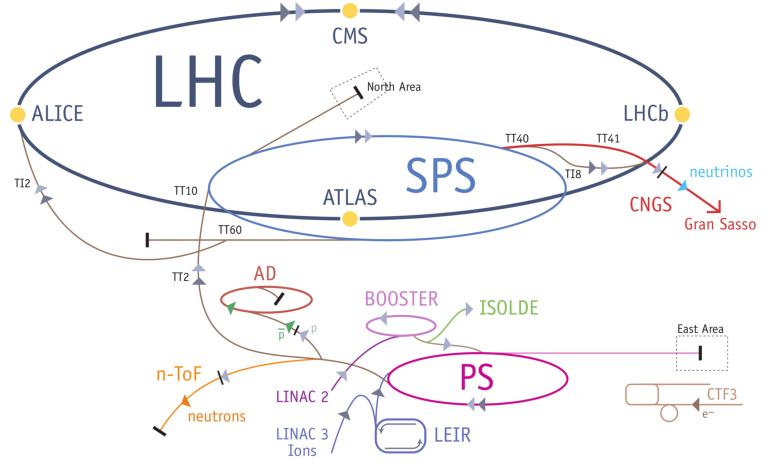
\includegraphics[width=.5\textwidth]{lhc_injection.pdf}
  \caption{Ligne d'injection du LHC. Figure tiré de la
    référence~\cite{Lefevre:1165534}}
  \label{fig:lhc_injection}
\end{figure}

\section{Le détecteur ATLAS}
\label{sec:lhc_atlas:atlas}

Le détecteur ATLAS (figure~\ref{fig:atlas}), décrit en détail dans la
référence~\cite{collaboration_atlas_2008}, est un assemblage de quatre
grand sous-détecteurs. Le détecteur interne, composé de détecteurs
semi-conducteurs au silicium ainsi que d'un ensemble de tubes à
dérives, est décrit dans la
section~\ref{sec:lhc_atlas:atlas:indet}. Les calorimètres
électromagnétiques et hadroniques sont traités dans la
section~\ref{sec:lhc_atlas:atlas:calo}, le spectromètre à muons dans
la section~\ref{sec:lhc_atlas:atlas:mu}. Finalement le système
d'acquisition des données est décrit dans la
section~\ref{sec:lhc_atlas:atlas:daq}.

\begin{figure}[h]
  \centering
  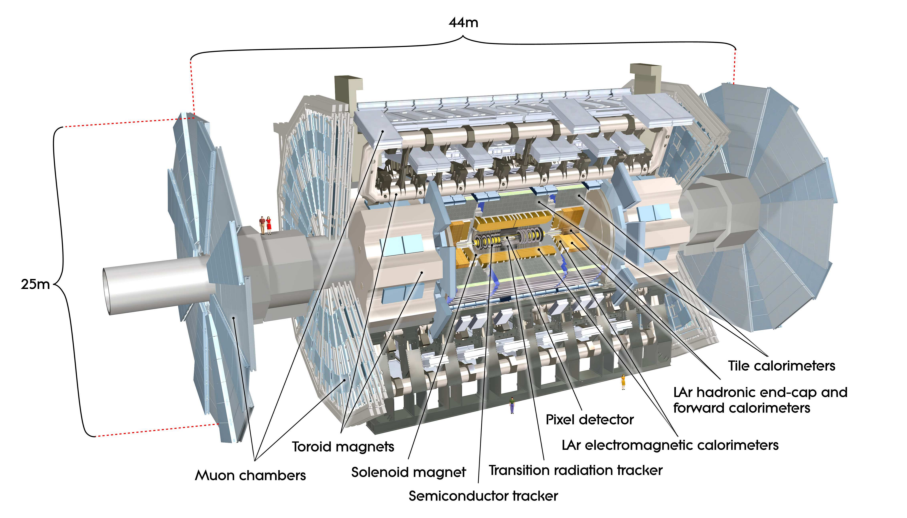
\includegraphics{atlas.pdf}
  \caption{Le détecteur ATLAS. Figure tirée de la référence~\cite{collaboration_atlas_2008}.}
  \label{fig:atlas}
\end{figure}

\subsection{Préambule: système d'unités}
\label{sec:units}

Le système d'unité couramment utilisé pour décrire le détecteur ATLAS
et les interactions qui s'y produise a son origine au point
d'interaction. L'axe $z$ est dans la direction du faisceau, l'axe $x$
pointe vers le centre de l'anneau formé par le tunnel du LHC et l'axe
$y$ est orienté vers le haut. Le plan $x-y$ défini la direction
transverse, dans laquelle plusieurs quantité sont calculées puisque
l'impulsion initiale y est nulle. L'angle dans ce plan, donc autour de
l'axe $z$, est noté $\phi$.

Il est possible d'associer une \emph{rapidité}
$y = \frac{1}{2}ln((E + p_Z)/(E - p_Z))$ aux objets massifs. Il est
commun d'utiliser une paramétrisation de cette quantité, la
\emph{pseudo-rapidité}, définie en fonction de l'angle polaire
$\theta$ (mesuré à partir de l'axe~$z$), $\eta =
-ln(tan(\theta/2))$. Cette coordonnée est très utile puisque la
section efficace différentielle de la production de gerbes est
approximativement constante en $\eta$l~\cite{thomson_modern_2013}. Les
directions dans le plan $y-z$ définies par quelques valeurs de $\eta$
sont montrés dans la figure~\ref{fig:eta}. La distance entre
différents objets est souvent défini dans l'espace $\eta-\phi$:
$\Delta R = \sqrt{\Delta\eta^2 + \Delta\phi^2}$.
\begin{figure}[h]
  \centering
  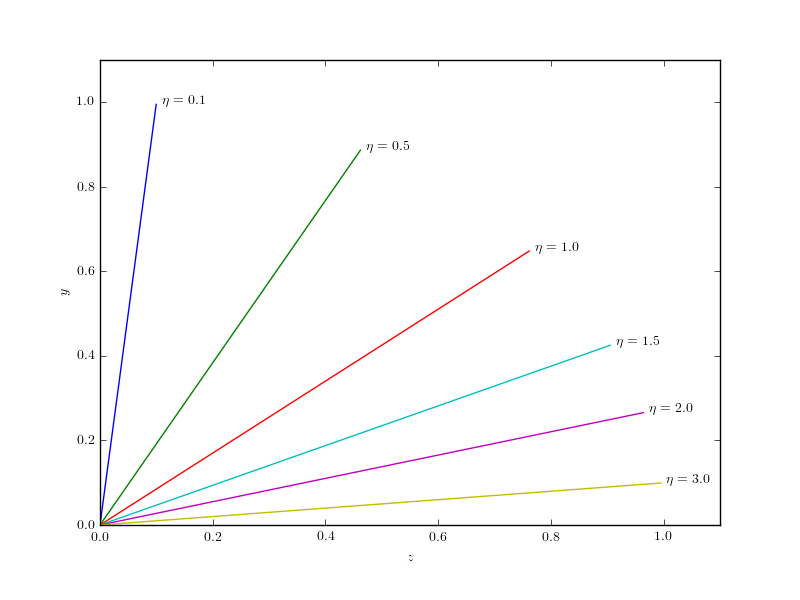
\includegraphics[width=.5\textwidth]{eta.png}
  \caption{Directions définies par quelques valeurs de $\eta$ dans le plan $y-z$.}
  \label{fig:eta}
\end{figure}

\subsection{Le détecteur interne}
\label{sec:lhc_atlas:atlas:indet}

% Critères

\subsubsection{PIXEL}

Le détecteur PIXEL est la composante d'ATLAS la plus près du
faisceau. Il s'agit de trois assemblages cylindriques coaxiaux au
centre et trois disques aux extrémités munis de senseurs en silicium
segmentés en pixels. Le PIXEL permet donc d'obtenir la distribution en
deux dimensions des dépôts de charges engendrés par les particules
chargés traversant le détecteur.

À cause des haut taux de productions de particules produites lors de
l'opération du LHC à luminosité maximale et à cause de sa proximité au
sommet d'interaction, le PIXEL doit être exceptionnellement résistant
à la radiation ionisante qui pourrait dégrader sa performance. Il doit
aussi avoir une résolution exceptionnelle, même à haut taux
d'occupation, pour permettre une performance optimale lors du
retraçage~\footnote{De l'anglais, \emph{tracking}} et de la mesure des
coordonnées du sommet d'interaction. Ces besoins particuliers motivent
l'utilisation d'une technologie innovatrice peu conventionnelle: à
partir d'une brique de silicium de type $n$ (excès de donneurs
d'électrons), on applique un implant $p$ (excès d'accepteurs) d'un
côté et implant $n^+$ de l'autre. Ce choix particulier permet aux
senseurs d'opérer correctement même longtemps après que les dépôts de
charges dans le silicium aient occasionné une inversion de type de la
brique de $n$ vers $p$. De plus, le silicium utilisé est fortement
oxygéné, ce qui permet de diminuer les dommages dûs à la radiation
incidente~\cite{collaboration_atlas_2008}.

Souvent, le passage d'une particule chargée à travers un senseur du
PIXEL illumine plus d'un pixel. Ce phénomène est due, entre autre, à
la dérive des électrons dans au champ magnétique axial du détecteur
interne, aux rayons-$\delta$ (électrons éjectés de leurs sites) et au
fait que deux particules peuvent passer simultanément très près les
unes des autres lors de collisions à haute luminosité. Cette dernière
situation peut avoir un effet dramatique sur la précision de
l'estimation de position des particules et arrive fréquemment dans les
gerbes hadroniques de très hautes énergies. Pour mitiger ce problème,
un algorithme utilisant des réseaux de neurones (voir
section~\ref{sec:susy_atlas:dl:ml}) est utilisé pour estimer le nombre
de particule dans chaque groupe de pixels contiguës ainsi que leurs
positions~\cite{collaboration_neural_2014}, permettant de quasiment
retrouver la résolution de conception optimale, soit $10~\mu$m dans la
direction $x$ locale ($R-\phi$ globale) et $115~\mu$m dans la
direction $y$ locale ($z$ globale), comme le montre la
figure~\ref{fig:pixel_acc}.

\begin{figure}
  \centering
  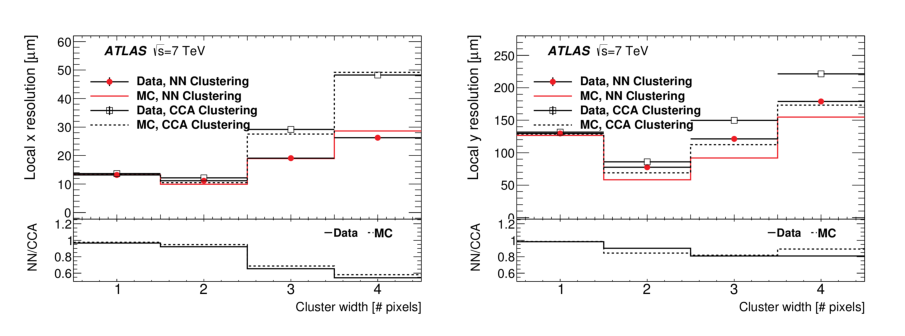
\includegraphics{pixel_acc.pdf}
  \caption{Résolution de la position des particules passant à travers
    le détecteur pixel en fonction du nombre de pixel contiguës
    illuminés, dans les directions $x$ locales ($R-\phi$ globales) (à
    gauche) et $y$ locales ($z$ globale) (à droite), selon que
    l'algorithme de réseaux de neurones est utilisé ou non. Figure
    tirée de la référence~\cite{collaboration_neural_2014}}
  \label{fig:pixel_acc}
\end{figure}

%% IBL
Outre les grandes doses de radiations ionisantes absorbées par les
trois couches du PIXEL, des déficiences importantes dans
l'électronique des senseurs peuvent apparaître éventuellement et sont
très difficile, voir impossible, à réparer. Lorsque de tels dommages
affectent la couche la plus près du points d'interaction, la
\emph{couche-B} situé à $\approx 50$~mm du centre, la performance du
retraçage peut être sérieusement dégradés. Au moment de la
construction du détecteur, il n'y avait cependant pas assez de place
entre la couche-$B$ et le tuyau de la ligne de faisceau pour y
installer une couche additionnelle. Or, une contrainte importante
dans le choix de ce rayon est l'instabilité du plancher de la caverne
ATLAS, qui avait été estimé à environ 5~mm. Or, des mesures effectués
entre 2003 et 2007 on démontré que cette instabilité est plutôt de
l'ordre de 1~mm, ce qui permettrait de réduire la ligne de faisceau de
4~mm, donnant alors assez de jeu pour pouvoir installer une couche
additionnelle~\cite{capeans_atlas_2010}. C'est précisément ce qui a été
fait en 2014, lors de la première grande mise-à-niveau du détecteur,
avec l'installation du \emph{IBL} (\emph{Insertable B-Layer}) (voir
figure~\ref{fig:ibl}). Avec cette couche additionnelle, l'estimation de
la position du sommet d'interaction est grandement améliorée.

\begin{figure}[h!]
  \centering
  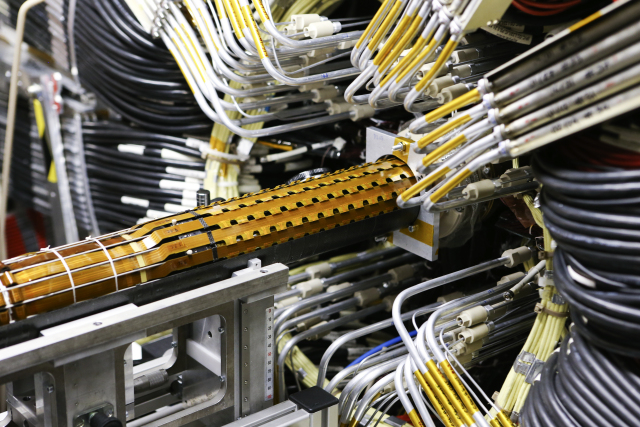
\includegraphics{ibl.jpg}
  \caption{Image de l'installation du IBL en 2014. Figure tirée de la référence~\cite{MarcelloniDeOliveira:1702006}}
  \label{fig:ibl}
\end{figure}

% SCT
\subsubsection{SCT}

Au dessus du pixel se trouve le \emph{Semiconductor Tracker}, ou SCT,
un ensemble de 4 assemblages cylindriques au centre et de quatre
disques aux extrémités munis de plusieurs senseurs à micro-bandes de
silicium. À la différence d'un senseur à pixel, les senseurs sont
implantés en bandes parallèles sur la plaque de silicium, et donc
chaque module fourni une mesure de position dans une seule
direction. Pour obtenir de l'information dans les deux directions ($z$
et $R-\phi$), les modules sont installés en paires séparés par un
angle de 40~mrad, comme le montre la figure~\ref{fig:sct}, définissant
une grille en 2 dimensions.

\begin{figure}[h]
  \centering
  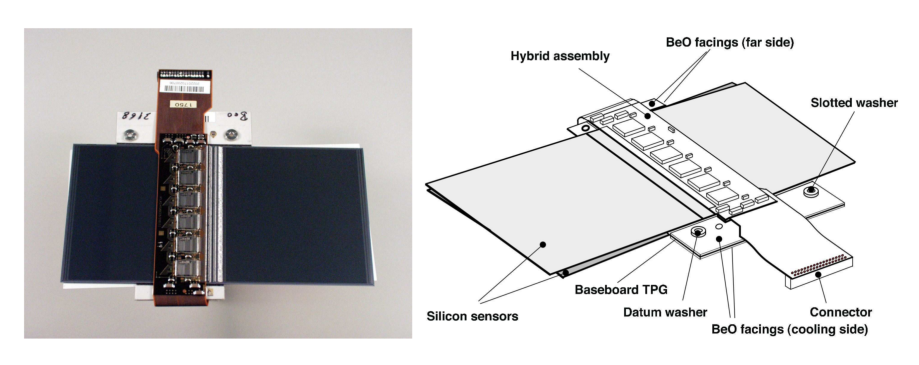
\includegraphics{sct.pdf}
  \caption{Photographie d'un module du SCT (à droite) et schéma
    correspondant (gauche). On y voit l'angle relatif entre les deux
    plaques de silicium. Figure tirée de la
    référence~\cite{collaboration_atlas_2008}}
  \label{fig:sct}
\end{figure}

La précision des mesures du SCT est de 17~$\mu$m dans la direction
$R-\phi$ et de 580~$\mu$m dans la direction $z$. Ces mesures sont
moins précises que celles du PIXEL, mais le SCT fourni quatre mesures
additionnelles de position à relativement bonne précision et à moindre
coût qu'un détecteur de type pixel de taille comparable, représentant
un bon compromis pour améliorer la performance du retraçage.


% TRT

\subsubsection{TRT}

Le détecteur interne est complété par le \emph{Transition Radiation
  Tracker}, ou TRT, un ensemble de tubes à dérives. Les tubes de 4~mm
de diamètres en polyimide sont recouvert à l'intérieur d'une couche
d'aluminium, définissant ainsi la cathode. Au centre se trouve un fil
de tungstène plaqué avec de l'or, définissant l'anode. Une différence
de potentiel de $\approx -1500$~V est appliquée entre l'anode et la
cathode. Les tube sont remplis d'un mélange de xénon ou d'argon, de
CO$_2$ et d'O$_2$. Le TRT est divisé en trois sections:
une section centrale cylindrique avec des tubes parallèles au faisceau
séparés en deux au centre et deux disques aux extrémités avec des
tubes dans la direction radiale.

Lorsqu'une particule chargée Passe à travers un tube, elle ionise le
mélange gazeux et amorce une cascade d'électrons et d'ions qui
dérivent vers l'anode et la cathode, créant ainsi un signal. La forme
du signal est analysée pour mesurer le temps de dérive de la cascade
qui, avec une calibration appropriée %(voir figure~\ref{fig:trt})
,
permet de mesurer la distance entre la particule et l'anode. La
position de l'anode étant précisément connue, cela permet donc de
mesurer une position en $R-\phi$ avec une précision de 130~$\mu$m.

% \begin{figure}[h]
%   \centering
%   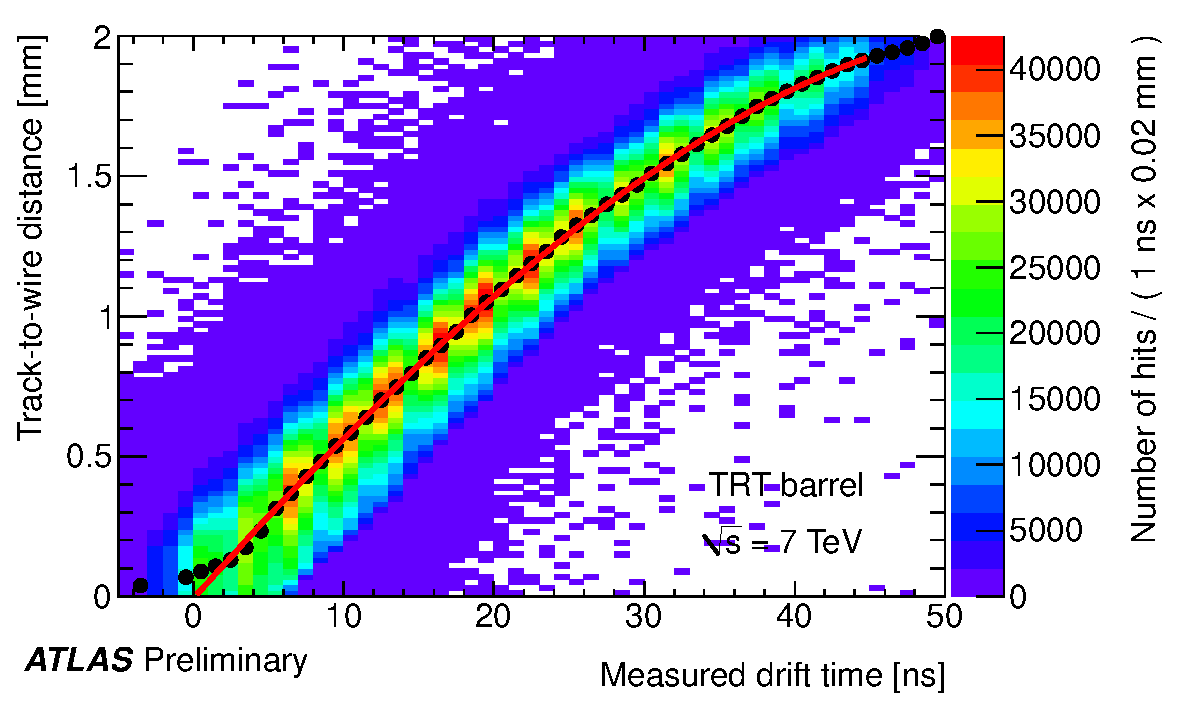
\includegraphics[width=0.5\textwidth]{trt.pdf}
%   \caption{Relation entre le temps de dérive et la distance par
%     rapport à l'anode dans le TRT. Figure tirée de la
%     référence~\cite{ATLAS-CONF-2011-006}}
%   \label{fig:trt}
% \end{figure}

%% electron ID
Lorsqu'une particule chargée traverse l'interface entre deux milieux
ayant des constantes diélectriques différentes, ce qui peut engendrer
de la radiation de transition sous forme de photons. Cet effet est
exploité dans le TRT pour identifier les électrons: les électrons
produisent des photons en entrant dans un des tube, les photons
interagissent avec le gaz pour créer une cascade d'électron dont la
charge totale est au-dessus de celle directement engendré par
l'électron. Deux seuils sont alors défini: un seuil bas, pour séparer
les signaux d'ionisation directe du bruit et un seuil haut, pour
reconnaître les signaux venant de radiation de transition et optimisé
pour reconnaître les électrons parmi des pions chargés.

\subsubsection{Retraçage}

Les trois sous-systèmes du détecteur interne servent à permettre de
retracer précisément le passage de particules chargés à travers le
détecteur pour mesurer la position du sommet d'interaction et
l'impulsion des particules. Le détecteur interne étant plongé dans un
champ magnétique axial de 2~T, les particules chargés produites lors
de collisions suivent une trajectoire hélicoïdale dont le rayon est
proportionnel à l'impulsion. L'erreur sur l'estimation de l'impulsion
dépend à la fois de la précision des mesures individuelles de
positions, de leurs nombres ainsi que de la longueur totale de la
trace~\cite{olive_detectors_2014}. Ainsi, le détecteur PIXEL donne
trois mesures très précises, le SCT en rajoute 4 avec un peu moins de
précision. Le TRT est beaucoup moins précis que les deux autres mais
rajoute environ 36 mesures par trace.

\subsection{Les calorimètres}
\label{sec:lhc_atlas:atlas:calo}

Au-dessus du détecteur interne se trouvent les calorimètres
électromagnétiques et hadroniques d'ATLAS. Comme les sous-systèmes du
détecteur interne, ils sont chacun séparés en une partie centrale
cylindrique ainsi que deux disques à grand $|\eta|$. \\

Le calorimètre électromagnétique est un calorimètre à échantillonnage
avec absorbeurs en plomb et couches actives en argon liquide. Les
couches actives sont en formes d'accordéon pour avoir une couverture
sans interruption en $\phi$. 

Un détecteur constitué d'un couche
d'argon liquide d'une profondeur de 1.1~cm dans la partie centrale et
de 0.5~cm aux extrémités est installé devant le calorimètre
électromagnétique et sert à mitiger les pertes d'énergies encourus par
les particules chargés avant d'atteindre le
calorimètre~\cite{andrieux_construction_2002}. \\

Directement au-dessus de la partie centrale du calorimètre
électromagnétique se trouve le calorimètre hadronique à tuile,
constitués d'absorbeurs en acier et utilisant des scintillateurs pour
échantillonner l'énergie. Aux extrémités se trouvent deux calorimètres
cuivre-argon~liquide servant à la calorimétrie hadronique à grand
$|\eta|$ ($1.5 < |\eta| < 3.1$). Dans la région $3.1 < |\eta| < 4.9$
se trouve un autre calorimètre, le \emph{FCal}~\footnote{De l'anglais,
  \emph{Forward Calorimeter.}}. Les couches actives sont en argons
liquide et les couches passives en cuivre (première section, optimisée
pour calorimétrie électromagnétiques) ou en tungstène (deux sections
suivantes, optimisées pour calorimétrie hadronique).

\subsection{Le spectromètre à muon}
\label{sec:lhc_atlas:atlas:mu}

Les particules chargées perdent de l'énergie en interagissant avec le
milieu selon l'équation de Bethe-Bloch, montrée dans la
figure~\ref{fig:bethe-bloch}. Il existe un régime,
$1 \le\beta\gamma\le 10$ (approximativement), pour lequel la perte
d'énergie est à un minimum. Une particule dans ce régime est à son
minimum d'ionisation. Il se trouve que la grande majorité des muons
produits dans les collisions au LHC sont près du minimum d'ionisation
et donc sont les seules particules chargés qui traversent les
calorimètres sans être arrêtés, ce qui motive l'installation de
détecteurs dédiés aux muons au-delà des calorimètres, permettant
d'améliorer substantiellement l'identification et la précision des
mesures d'impulsions des muons.

\begin{figure}
  \centering
  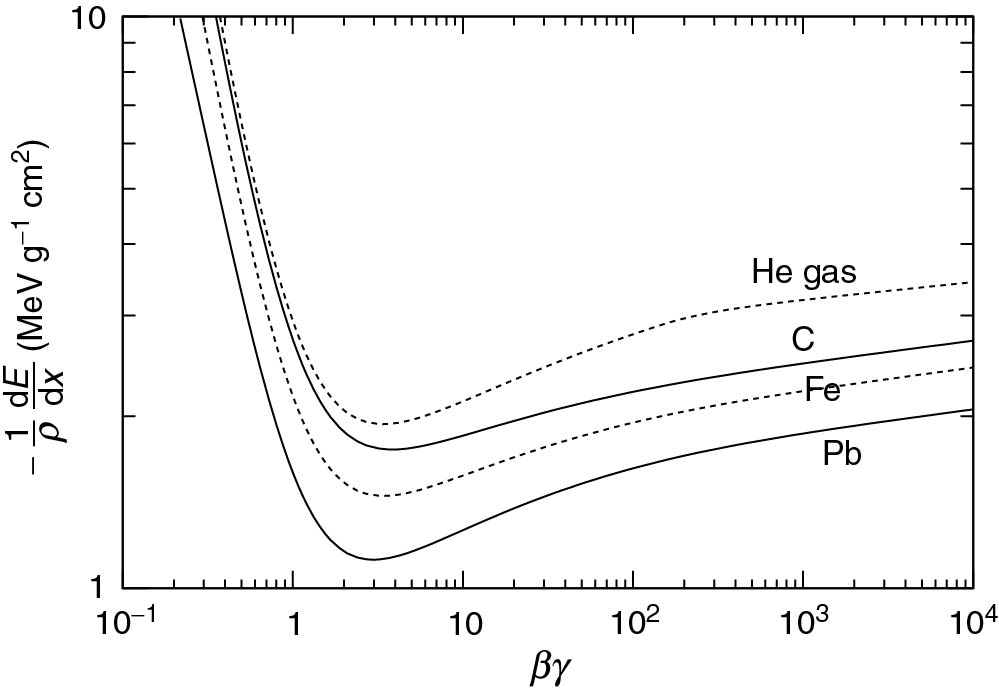
\includegraphics{bethe_bloch.jpg}
  \caption{Équation de Bethe-Bloch, qui exprime la perte d'énergie
    d'une particule chargée en fonction de sa vitesse dans différents
    milieux. Figure tirée de la référence~\cite{thomson_modern_2013}}
  \label{fig:bethe-bloch}
\end{figure}

Le détecteur ATLAS est complété par l'ajout de trois aimants toroïdaux
(un aimant central, deux aux extrémités derrière les calorimètres) et
par des ensembles de chambres à muons . Dans la partie centrale, les
chambres sont disposés en-dessous, à l'intérieur et au-dessus de
l'aiment toroïdal central. Aux extrémités se trouvent de grands
disques comme montré dans la figure~\ref{fig:atlas}.

\subsection{Déclencheurs}
\label{sec:lhc_atlas:atlas:daq}

À luminosité maximale il y a à peu près 1 milliard de collisions par
secondes ce qui correspond à une fréquence de 1~GHz. L'enregistrement
sur disque des données prises par le détecteur ATLAS nécessitant
environ 1.3~Mb par événement, un stockage complet nécessiterait plus
de 1000~Tb/s de données enregistrés, ce qui est beaucoup trop élevé
pour être possible. De plus, seulement une petite fraction de ces
événements correspondent aux processus de nouvelle physique recherchés
par la collaboration. Le détecteur ATLAS est donc doté d'un système de
déclencheurs~\footnote{De l'anglais, \emph{triggers}} permettant de
limiter la fréquence d'enregistrement à 200~Hz. Il y a deux paliers de
déclencheurs: un niveau matériel et un niveau logiciel. Le premier
niveau est un ensemble de dispositifs installés directement sur le
détecteur et qui sont activés par plusieurs signaux, tels que le
passage de particules à haute impulsion transverse dans différentes
zones du détecteur ou encore un grand déficit d'impulsion transverse
dans une direction (calculée par conservation de l'impulsion). Ce
premier niveau défini des zones d'intérêts en $\eta-\phi$ qui sont
ensuite relayé à un ensemble de serveurs sur lesquels des logiciels
font une analyse plus détaillé pour déterminer si l'événement est
intéressant ou non~\cite{collaboration_atlas_2008}.

%%% Local Variables:
%%% mode: latex
%%% TeX-master: "memoire" 
%%% End:
